
We illustrate the phase-transition phenomena in finite dimensions with numerical experiments.
% We also demonstrate the fundamental trade-off between odds ratios and relative frequencies in association studies, as outlined in Proposition \ref{prop:signal-size-odds-ratio} and Corollary \ref{cor:signal-size-odds-ratio-conditional-frequency}, using evidence from large-scale genetic studies.

\subsection{The exact support recovery problem}

The sparsity and signal size of the sparse mean vector in the experiments are parametrized as in \eqref{eq:signal-sparsity} and \eqref{eq:signal-size}, with signal sizes assumed equal.
We estimate the support set $S$ with using Bonferroni's procedure, where the nominal FWER level for Bonferroni's procedures are set at $1/(5{\log{p}})$, in line with the assumptions in Theorem \ref{thm:chi-squared-exact-boundary}.
Experiments were repeated 1000 times at each of the 400 sparsity-and-signal-size combinations, for dimensions $p=10^2, 10^3$, and $10^4$.

The empirical probabilities of exact support recovery under Bonferroni's procedure are shown in Figure \ref{fig:phase-simulated-chi-squared}.
The numerical results suggest not only good accuracy of the predicted boundaries in high-dimensions ($p=10^4$, right panels of Figure \ref{fig:phase-simulated-chi-squared}), but also practical relevance even at moderate dimensions ($p=100$, left panels of Figure \ref{fig:phase-simulated-chi-squared}).

\begin{figure}
      \centering
      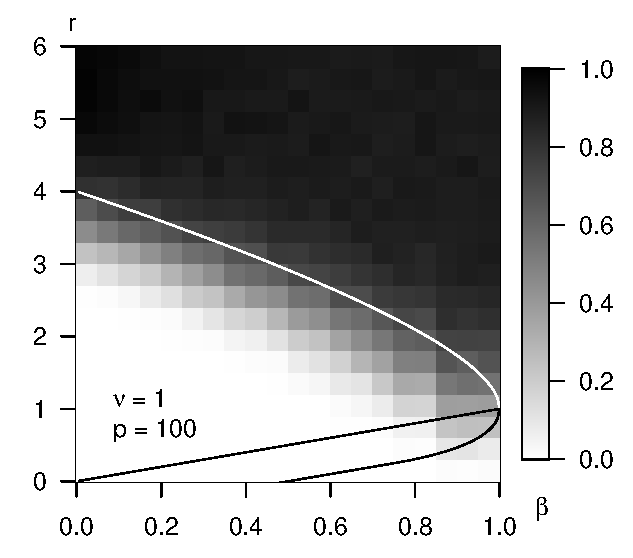
\includegraphics[width=0.32\textwidth]{./sim_strong_boundary/simulated_phase_diagram_chi-squared_nu1_p100.eps}
      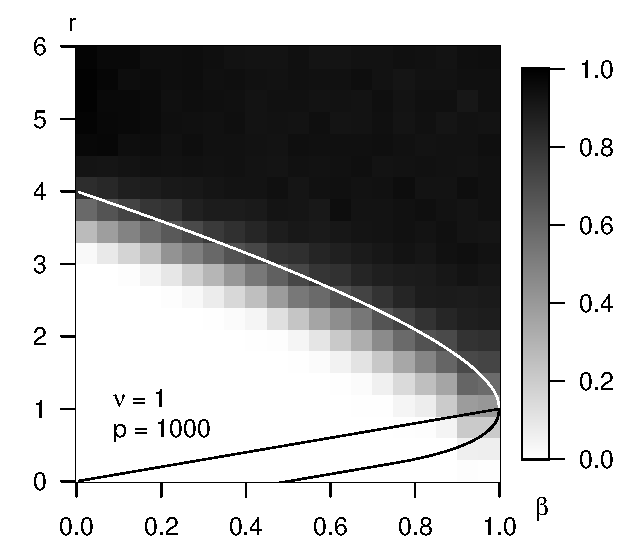
\includegraphics[width=0.32\textwidth]{./sim_strong_boundary/simulated_phase_diagram_chi-squared_nu1_p1000.eps}
      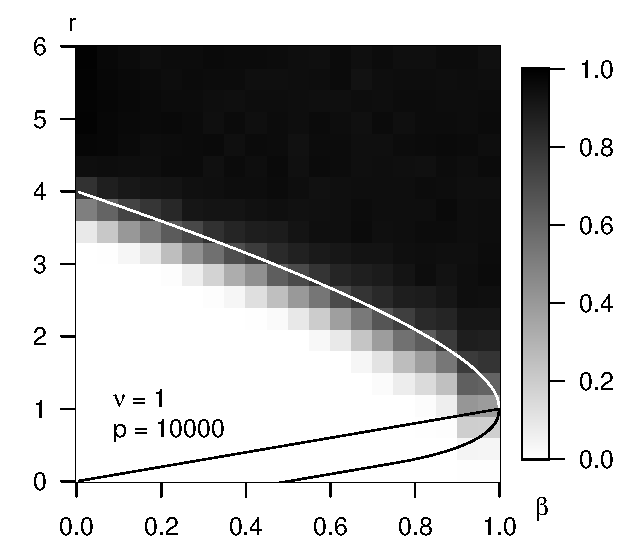
\includegraphics[width=0.32\textwidth]{./sim_strong_boundary/simulated_phase_diagram_chi-squared_nu1_p10000.eps}
      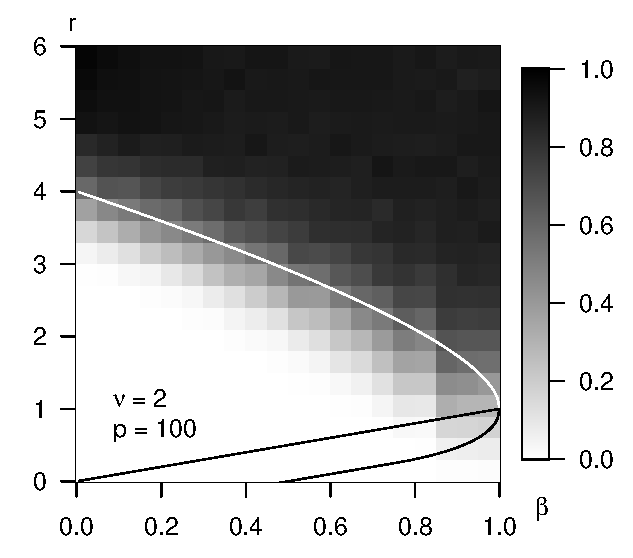
\includegraphics[width=0.32\textwidth]{./sim_strong_boundary/simulated_phase_diagram_chi-squared_nu2_p100.eps}
      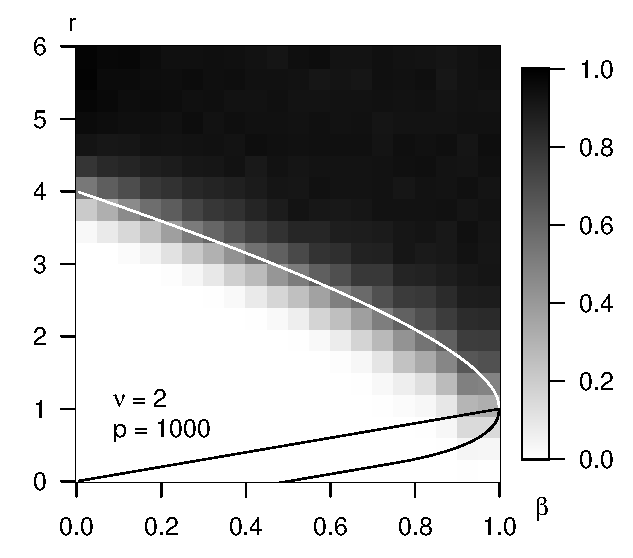
\includegraphics[width=0.32\textwidth]{./sim_strong_boundary/simulated_phase_diagram_chi-squared_nu2_p1000.eps}
      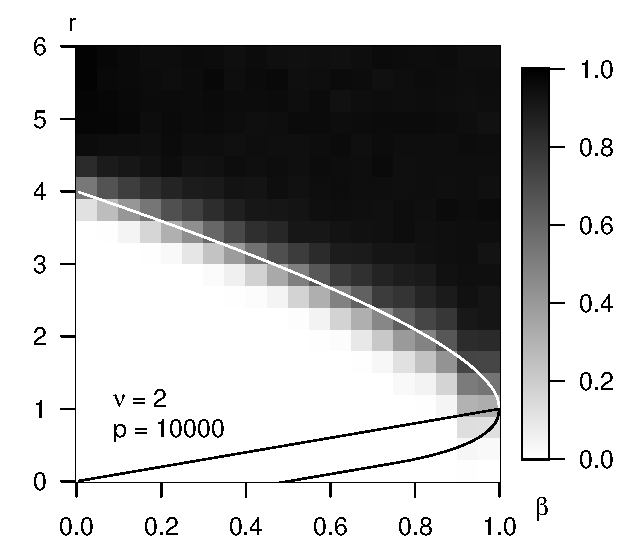
\includegraphics[width=0.32\textwidth]{./sim_strong_boundary/simulated_phase_diagram_chi-squared_nu2_p10000.eps}
      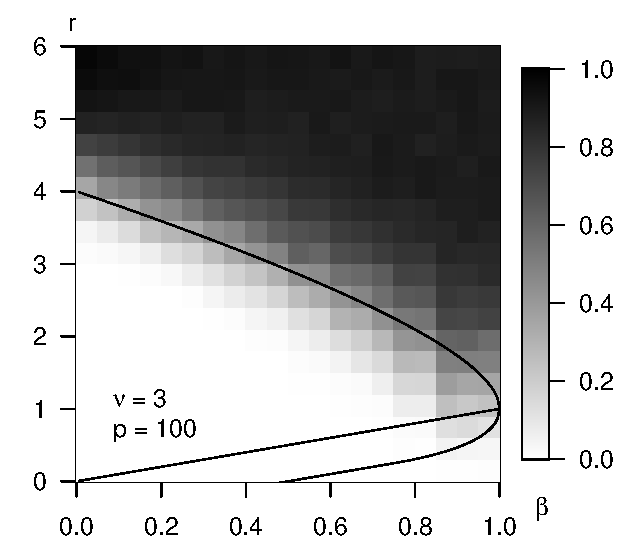
\includegraphics[width=0.32\textwidth]{./sim_strong_boundary/simulated_phase_diagram_chi-squared_nu3_p100.eps}
      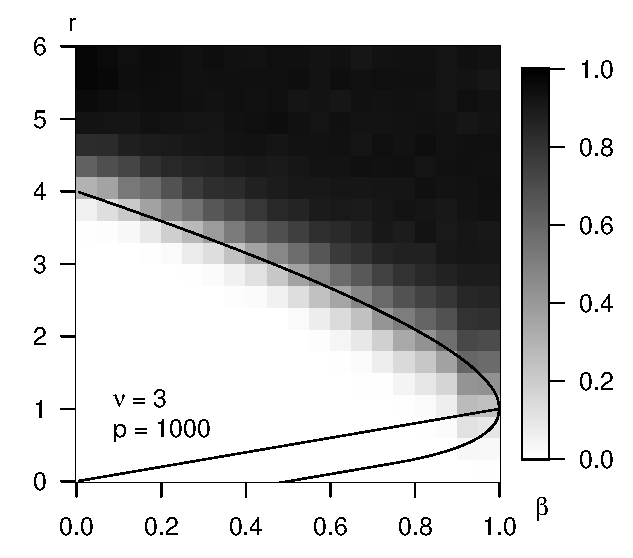
\includegraphics[width=0.32\textwidth]{./sim_strong_boundary/simulated_phase_diagram_chi-squared_nu3_p1000.eps}
      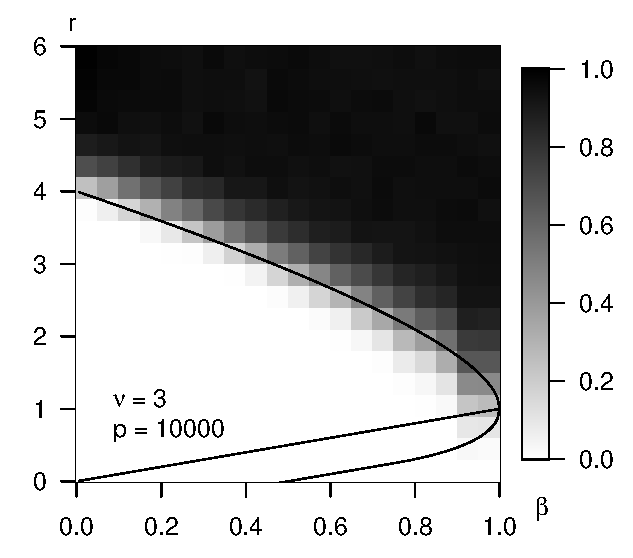
\includegraphics[width=0.32\textwidth]{./sim_strong_boundary/simulated_phase_diagram_chi-squared_nu3_p10000.eps}
      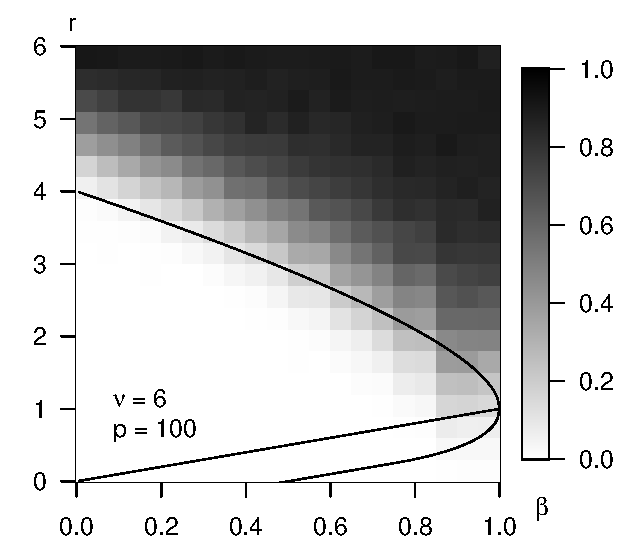
\includegraphics[width=0.32\textwidth]{./sim_strong_boundary/simulated_phase_diagram_chi-squared_nu6_p100.eps}
      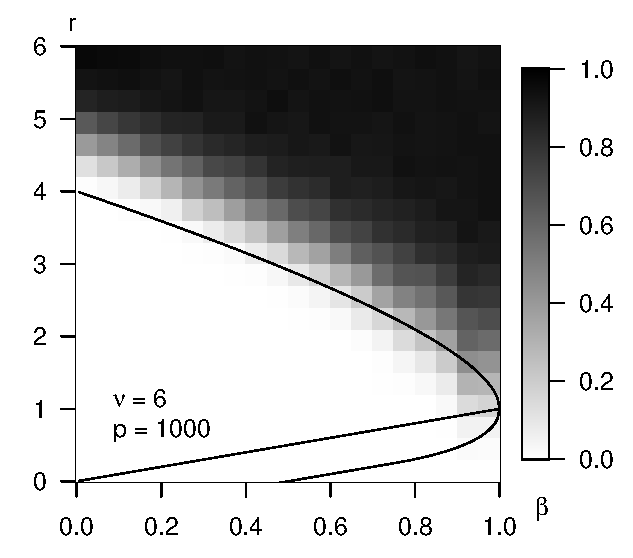
\includegraphics[width=0.32\textwidth]{./sim_strong_boundary/simulated_phase_diagram_chi-squared_nu6_p1000.eps}
      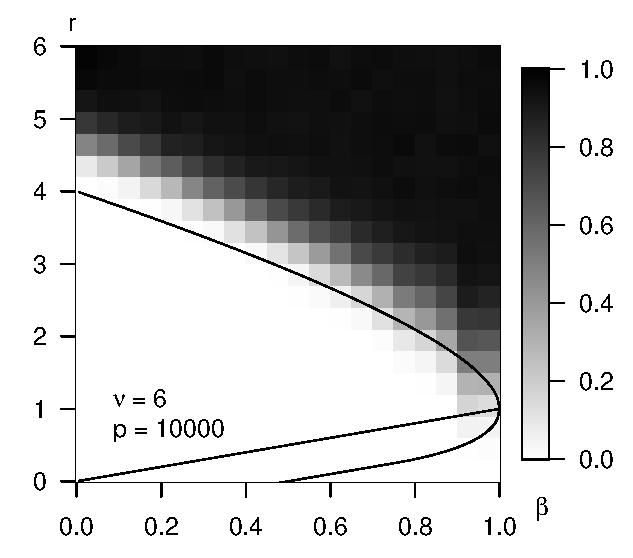
\includegraphics[width=0.32\textwidth]{./sim_strong_boundary/simulated_phase_diagram_chi-squared_nu6_p10000.eps}
      \caption{The empirical probability of exact support recovery using Bonferroni's procedure in the chi-squared model \eqref{eq:model-chisq}. 
      We simulate $\nu=1, 2, 3, 6$ (first to last row), at dimensions $p=10^2, 10^3, 10^4$ (left to right column), for a grid of sparsity levels $\beta$ and signal sizes $r$.
      The experiments were repeated 1000 times for each sparsity-signal size combination; darker color indicates higher probability of exact support recovery.  
      Numerical results are generally in agreement with the boundaries described in Theorem \ref{thm:chi-squared-exact-boundary}; for large $\nu$'s, the phase transitions take place somewhat above the predicted boundaries.
      The boundary for the approximate support recovery (Theorem \ref{thm:chi-squared-approx-boundary}) and the detection boundary (see \citep{donoho2004higher}) are plotted for comparison.} 
      \label{fig:phase-simulated-chi-squared}
\end{figure}

We conduct further experiments to examine the optimality claims in Theorem \ref{thm:chi-squared-exact-boundary} by comparing with the oracle procedure with thresholds $t_p=\min_{i\in S}x(i)$.
We also examine the claims in Remark \ref{rmk:strong-classification-boundary-1}, and compare the one-sided alternatives in Gaussian additive models with the two-sided alternatives (or equivalently, the chi-square model with $\nu=1$).
We apply both Bonferroni's procedure and the oracle thresholding procedure in both settings.

Experiments were repeated 1000 times for signal sizes ranging from $r=0$ to $6$, and for dimensions $10^2, 10^3$, and $10^5$.
Results of the experiments, shown in Figure \ref{fig:one-vs-two-sided-exact_support_recovery}, suggest vanishing difference between difficulties of two-sided vs one-sided alternatives in the additive error models, as well as vanishing difference between the powers of Bonferroni's procedures and the oracle procedures.

\begin{figure}
      \centering
      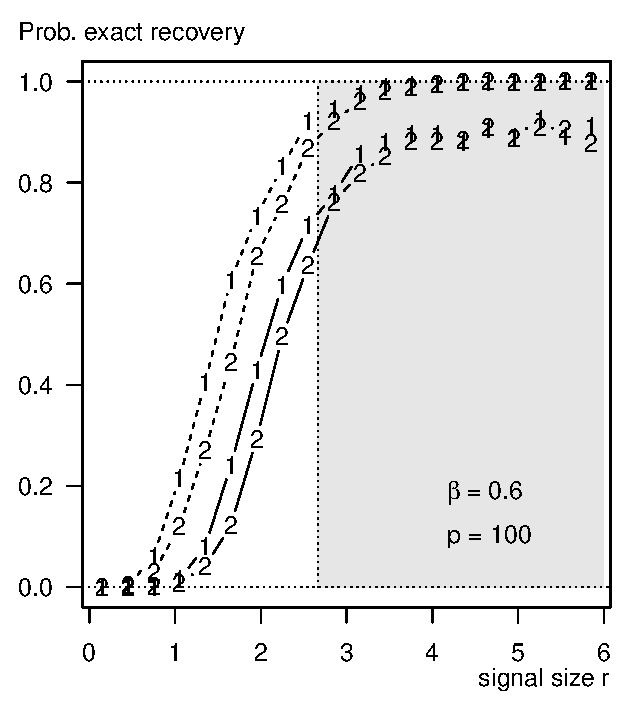
\includegraphics[width=0.32\textwidth]{./sim_one-vs-two-sided/exact_recovery_one-vs-two-sided_beta06_p100.eps}
      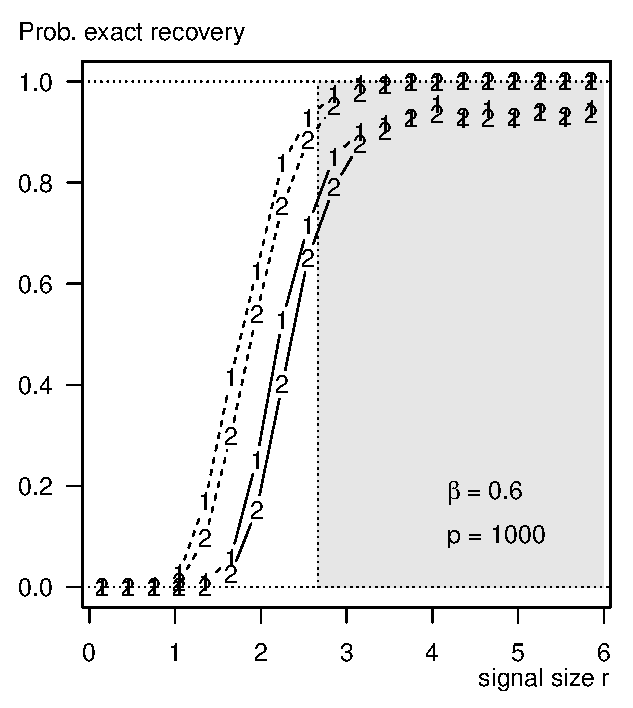
\includegraphics[width=0.32\textwidth]{./sim_one-vs-two-sided/exact_recovery_one-vs-two-sided_beta06_p1000.eps}
      % 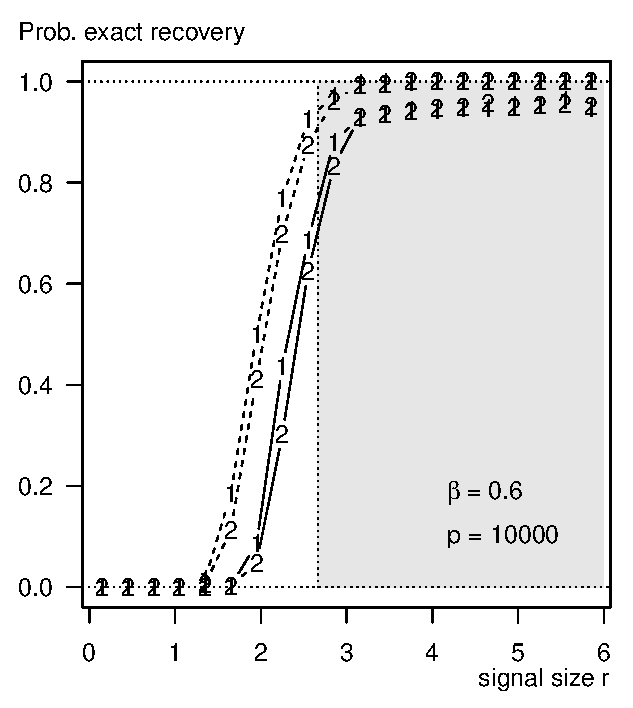
\includegraphics[width=0.33\textwidth]{./sim_one-vs-two-sided/exact_recovery_one-vs-two-sided_beta06_p10000.eps}
      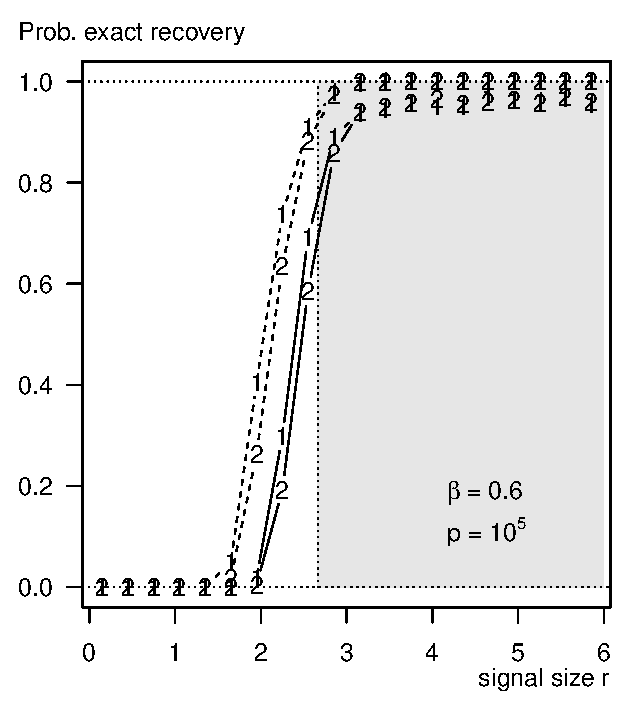
\includegraphics[width=0.32\textwidth]{./sim_one-vs-two-sided/exact_recovery_one-vs-two-sided_beta06_p100000.eps}
      \caption{The empirical probability of exact support recovery using Bonferroni's procedure (solid curves) and the oracle procedure (dashed curves) in the chi-squared model with $\nu=1$ (marked `2') and under one-sided alternatives in the additive Gaussian error model (marked `1'). 
      We simulate at dimensions $p=10^2, 10^3, 10^5$ (left to right) for a grid of signal sizes $r$ and sparsity level $\beta=0.6$.
      The experiments were repeated 1000 times for each method-model-signal-size combination. 
      Numerical results show evidence of convergence to the 0-1 law predicted by Theorem \ref{thm:chi-squared-exact-boundary}; regions where exact support recovery is asymptotically achievable are shaded in grey.
      The difference in power between Bonferroni's procedure and the oracle procedure, as well as in the two types of alternatives both decrease as dimensionality increases.} 
      \label{fig:one-vs-two-sided-exact_support_recovery}
\end{figure}

\subsection{The approximate, and approximate-exact support recovery problem}

Similar experiments are conducted to examine the optimality claims in Theorem \ref{thm:chi-squared-approx-boundary}, and in Remark \ref{rmk:weak-classification-boundary}.
The oracle procedure for approximate support recovery is defined to be the thresholding procedure with threshold
$$
t_p(x, S) \in \argmin_{t\in\R} \frac{|\widehat{S}(t)\setminus S|}{\max\{|\widehat{S}(t)|,1\}} + \frac{|S\setminus \widehat{S}(t)|}{\max\{|{S}|,1\}},
%\mathcal{R^\mathrm{oracle}} \in \argmin_{\widehat{S}(\mathcal{R})\in\mathcal{S}} \mathrm{risk}^{\mathrm{A}}(\mathcal{R}),
$$
where $\widehat{S}(t) = \{i\;|\;x(i)\ge t\}$;
in implementation, we need only scan the values of observations $t\in\{x(1), \ldots, x(p)\}$. 
The nominal FDR level for the BH procedure is set at $1/(5{\log{p}})$, satisfying the assumptions in Theorem \ref{thm:chi-squared-approx-boundary}; all other parameters are identical to that in the experiments for exact support recovery.
Results of the experiments are shown in Figure \ref{fig:one-vs-two-sided-approx_support_recovery} and Figure \ref{fig:phase-simulated-chi-squared-approx-boundary}.

We also examine the boundary described in Theorem \ref{thm:chi-squared-exact-approx-boundary}.
All experimental settings are identical to that in the experiments for approximate support recovery.
Results of the experiments are shown in Figure \ref{fig:phase-simulated-chi-squared-approx-exact-boundary}.
% Results for the BH procedure are in general close to that of the oracle procedure, 
We also compare the performance of the BH procedure with an oracle procedure with threshold
$$
t_p(x, S) \in \min_{i\in S} x(i).
$$
In experiments, we noticed that the BH procedure sets its threshold somewhat higher than the oracle, especially for small $\beta$'s. 
The phase transition for the oracle procedure (excluded in the interest of space) follows much more closely the predicted boundary \eqref{eq:approx-exact-boundary-chisquared}.

\begin{figure}
      \centering
      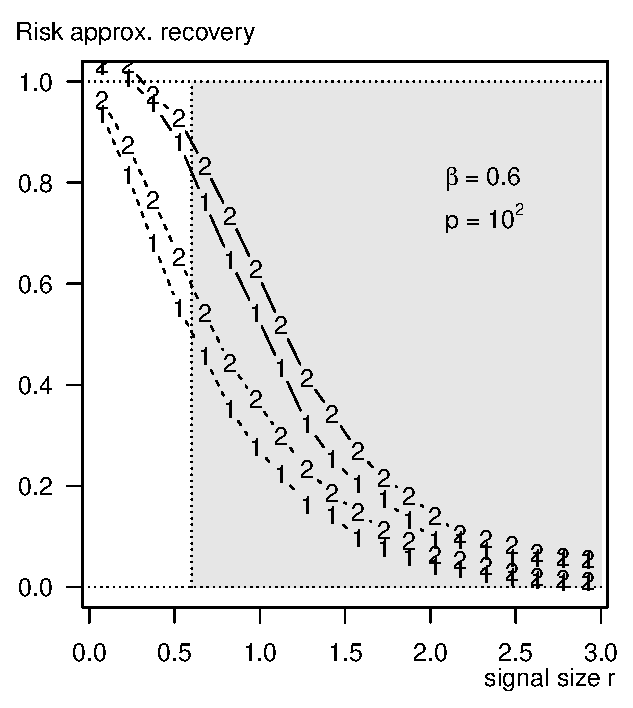
\includegraphics[width=0.32\textwidth]{./sim_one-vs-two-sided/approx_recovery_one-vs-two-sided_beta06_p100.eps}
      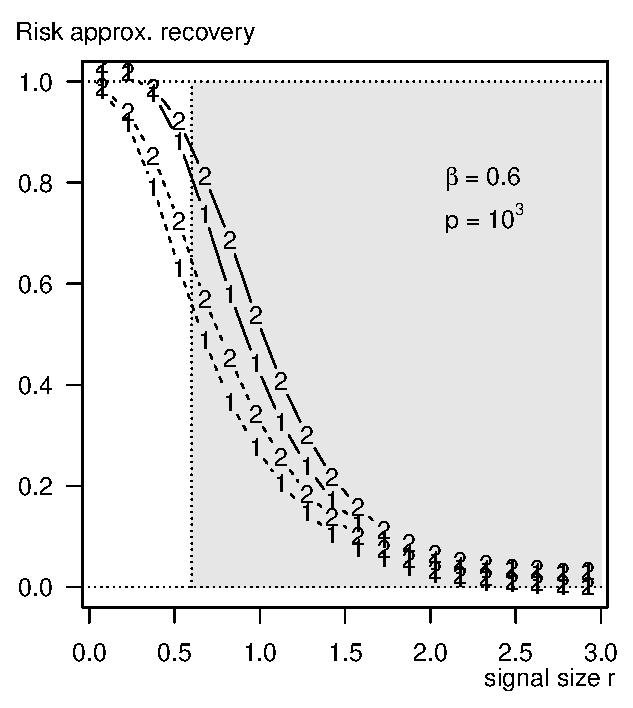
\includegraphics[width=0.32\textwidth]{./sim_one-vs-two-sided/approx_recovery_one-vs-two-sided_beta06_p1000.eps}
      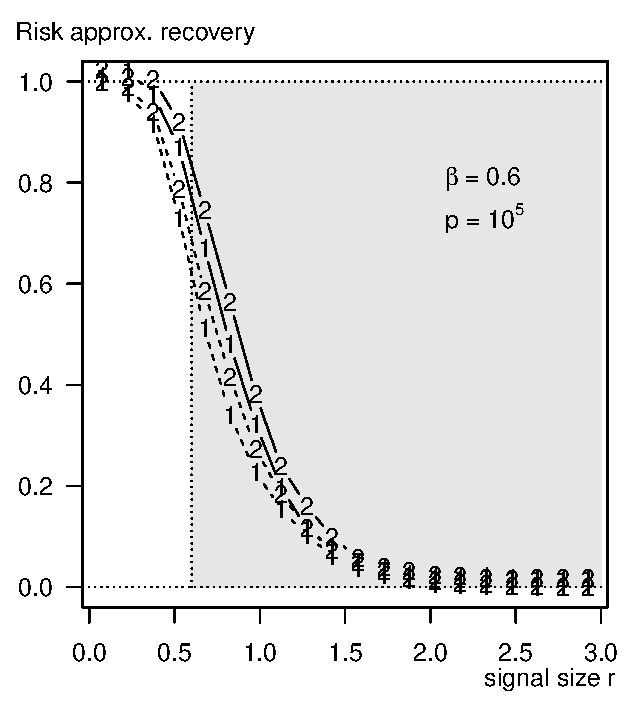
\includegraphics[width=0.32\textwidth]{./sim_one-vs-two-sided/approx_recovery_one-vs-two-sided_beta06_p100000.eps}
      \caption{The empirical risk of approximate support recovery using Benjamini-Hochberg's procedure (solid curves) and the oracle procedure (dashed curves) in the chi-squared model with $\nu=1$ (marked `2') and under one-sided alternatives in the additive Gaussian error model (marked `1'). 
      We simulate at dimensions $p=10^2, 10^3, 10^5$ (left to right) for a grid of signal sizes $r$ and sparsity level $\beta=0.6$.
      The experiments were repeated 1000 times for each method-model-signal-size combination. 
      Numerical results show evidence of convergence to the 0-1 law predicted by Theorem \ref{thm:chi-squared-approx-boundary}; regions where approximate support recovery is asymptotically achievable are shaded in grey.
      The difference in power between Benjamini-Hochberg's procedure and the oracle procedure, as well as in the two types of alternatives both decrease as dimensionality increases.} 
      \label{fig:one-vs-two-sided-approx_support_recovery}
\end{figure}


\begin{figure}
      \centering
      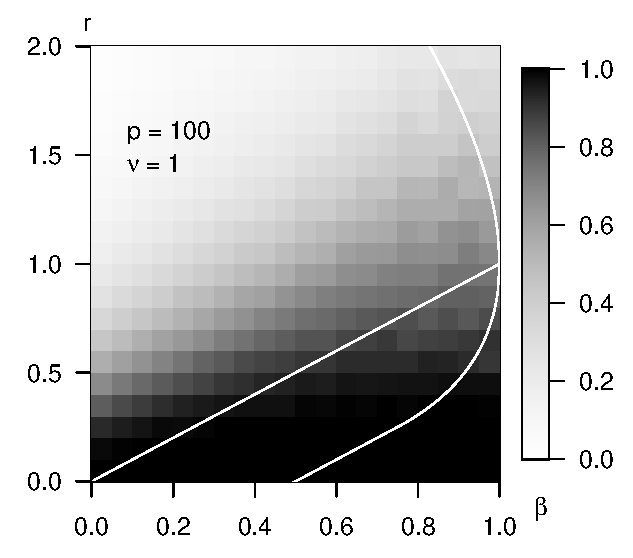
\includegraphics[width=0.32\textwidth]{./sim_weak_boundary/simulated_weak_boundary_chi-squared_nu1_p100.eps}
      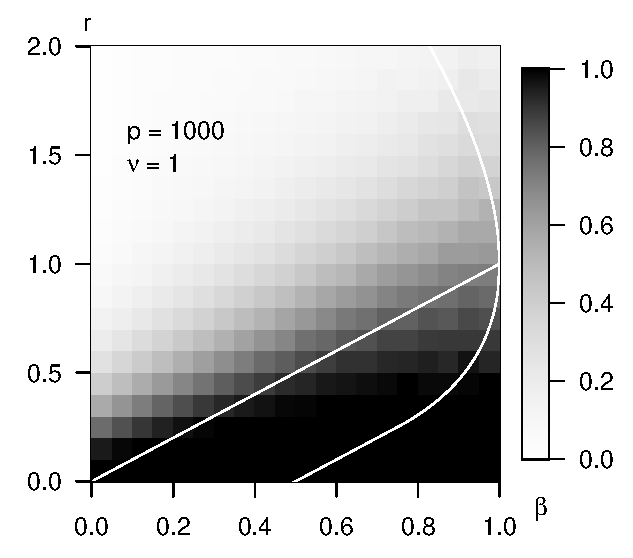
\includegraphics[width=0.32\textwidth]{./sim_weak_boundary/simulated_weak_boundary_chi-squared_nu1_p1000.eps}
      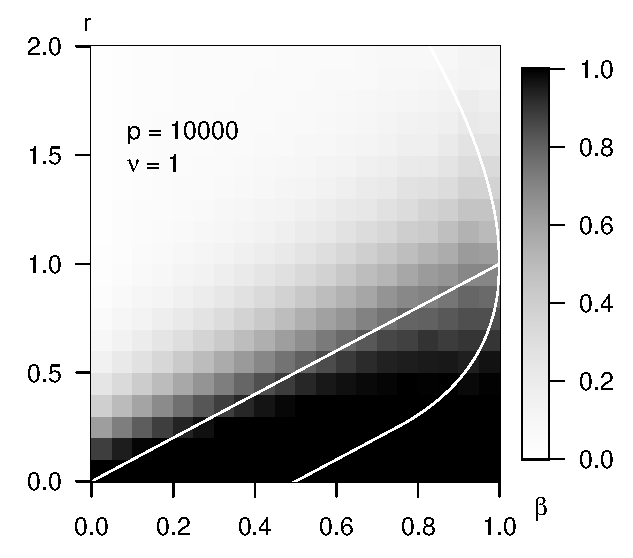
\includegraphics[width=0.32\textwidth]{./sim_weak_boundary/simulated_weak_boundary_chi-squared_nu1_p10000.eps}
      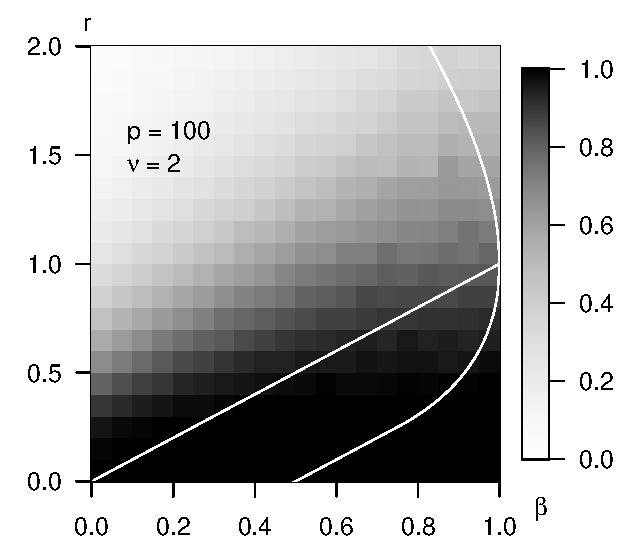
\includegraphics[width=0.32\textwidth]{./sim_weak_boundary/simulated_weak_boundary_chi-squared_nu2_p100.eps}
      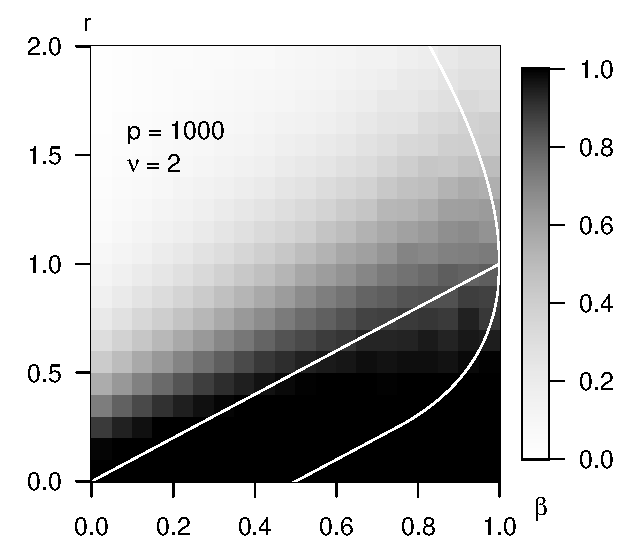
\includegraphics[width=0.32\textwidth]{./sim_weak_boundary/simulated_weak_boundary_chi-squared_nu2_p1000.eps}
      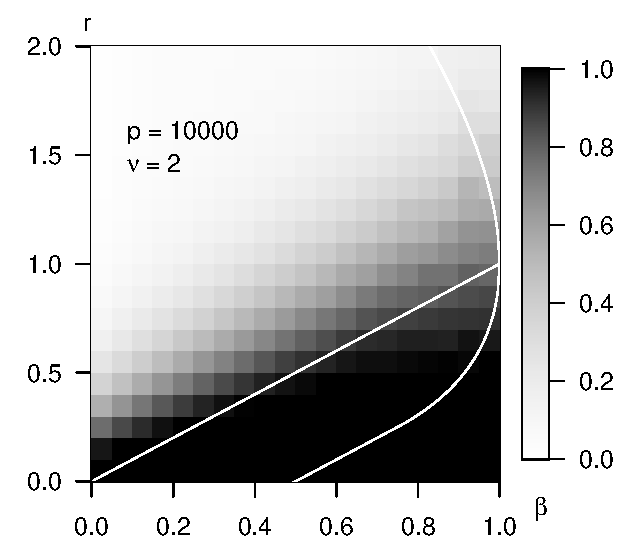
\includegraphics[width=0.32\textwidth]{./sim_weak_boundary/simulated_weak_boundary_chi-squared_nu2_p10000.eps}
      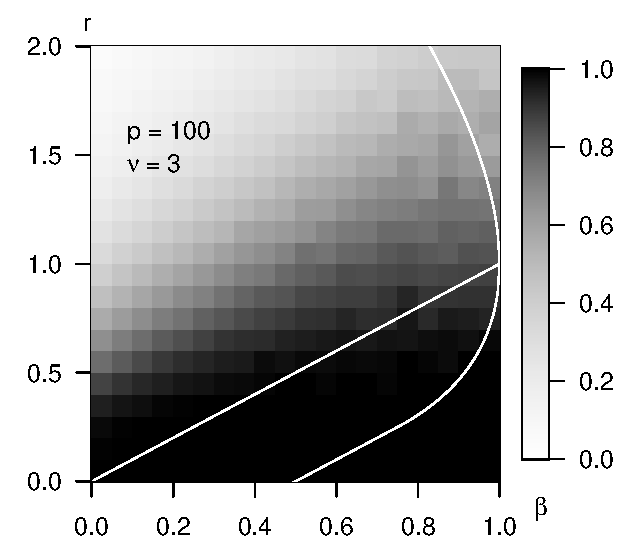
\includegraphics[width=0.32\textwidth]{./sim_weak_boundary/simulated_weak_boundary_chi-squared_nu3_p100.eps}
      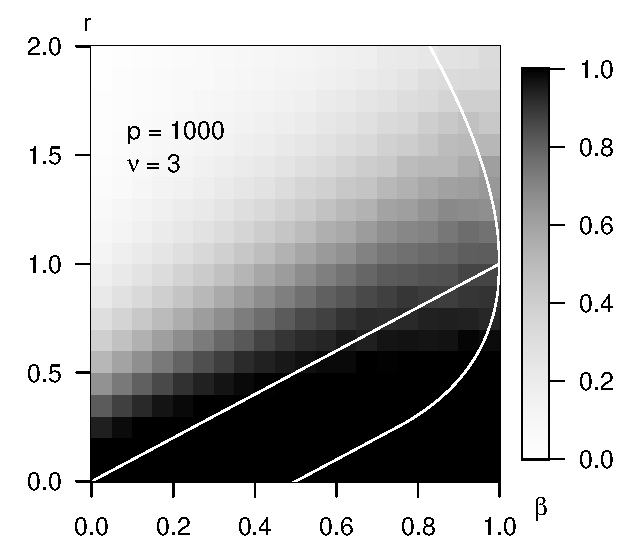
\includegraphics[width=0.32\textwidth]{./sim_weak_boundary/simulated_weak_boundary_chi-squared_nu3_p1000.eps}
      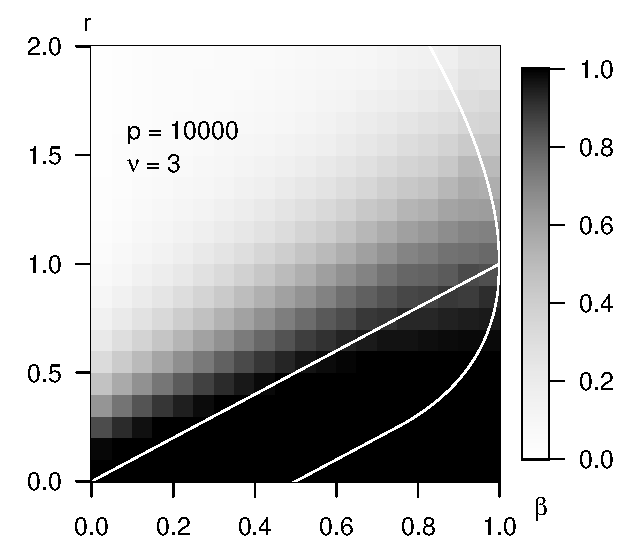
\includegraphics[width=0.32\textwidth]{./sim_weak_boundary/simulated_weak_boundary_chi-squared_nu3_p10000.eps}
      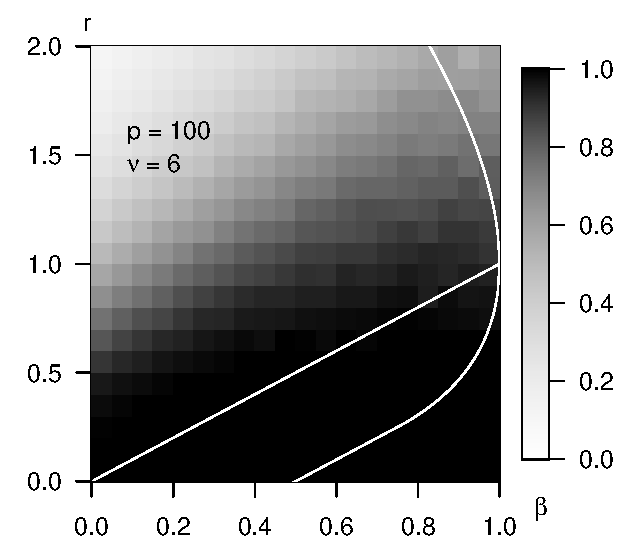
\includegraphics[width=0.32\textwidth]{./sim_weak_boundary/simulated_weak_boundary_chi-squared_nu6_p100.eps}
      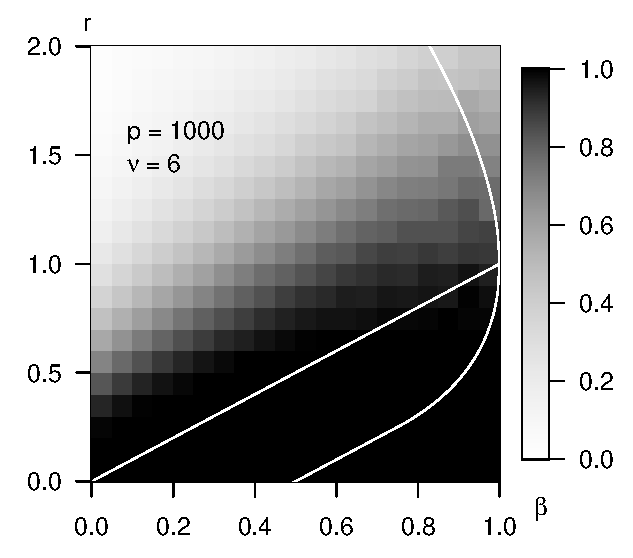
\includegraphics[width=0.32\textwidth]{./sim_weak_boundary/simulated_weak_boundary_chi-squared_nu6_p1000.eps}
      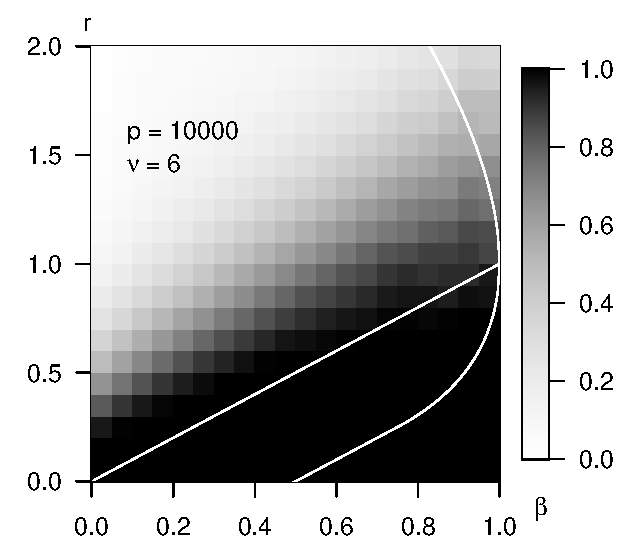
\includegraphics[width=0.32\textwidth]{./sim_weak_boundary/simulated_weak_boundary_chi-squared_nu6_p10000.eps}
      \caption{The estimated risk of approximate support recovery $\mathrm{risk}^{\mathrm{A}}$ (see \eqref{eq:risk-approximate}) of the Benjamini-Hochberg procedure in the chi-squared model \eqref{eq:model-chisq}. 
      We simulate $\nu=1, 2, 3, 6$ (first to last row), at dimensions $p=10^2, 10^3, 10^4$ (left to right column), for a grid of sparsity levels $\beta$ and signal sizes $r$.
      The experiments were repeated 1000 times for each sparsity-signal size combination; darker color indicates higher larger $\mathrm{risk}^{\mathrm{A}}$. 
      Numerical results are generally in agreement with the boundaries described in Theorem \ref{thm:chi-squared-approx-boundary}; for large $\nu$'s, the phase transitions take place somewhat above the predicted boundaries.
      The boundary for the exact support recovery problem (Theorem \ref{thm:chi-squared-exact-boundary}) and the detection boundary (see \citep{donoho2004higher}) are plotted for comparison.} 
      \label{fig:phase-simulated-chi-squared-approx-boundary}
\end{figure}


\begin{figure}
      \centering
      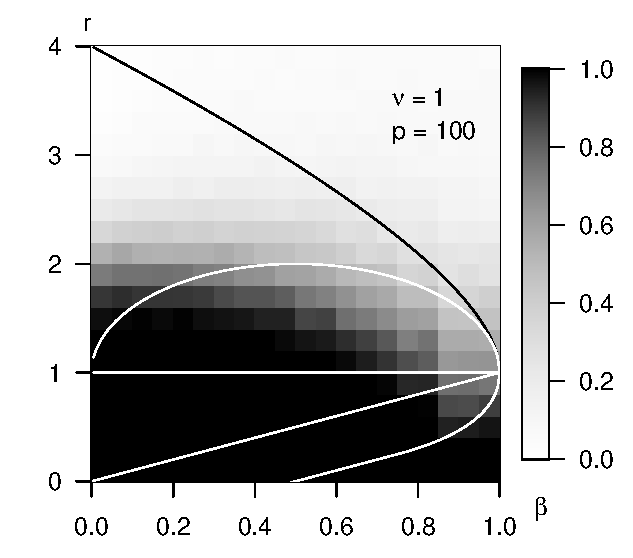
\includegraphics[width=0.32\textwidth]{./sim_approx-exact_boundary/simulated_approx-exact_boundary_chi-squared_nu1_p100.eps}
      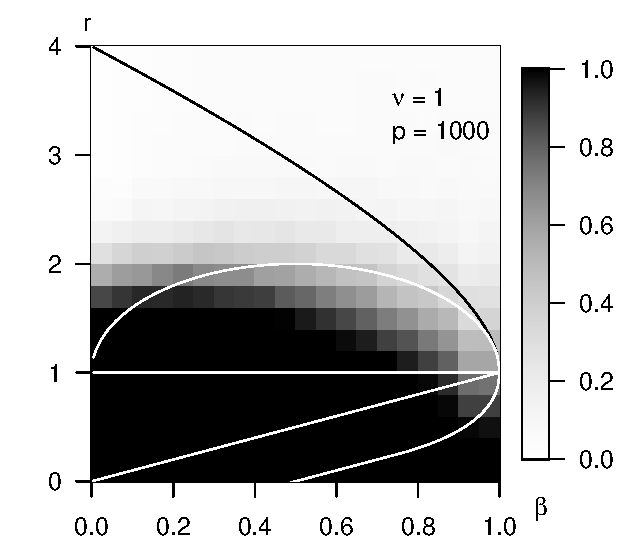
\includegraphics[width=0.32\textwidth]{./sim_approx-exact_boundary/simulated_approx-exact_boundary_chi-squared_nu1_p1000.eps}
      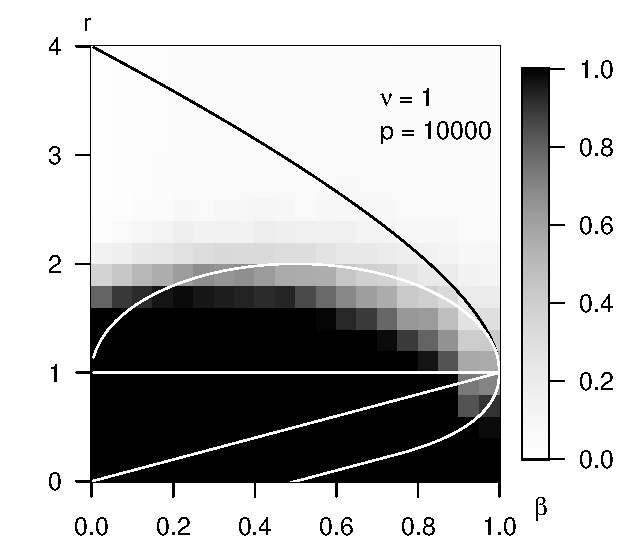
\includegraphics[width=0.32\textwidth]{./sim_approx-exact_boundary/simulated_approx-exact_boundary_chi-squared_nu1_p10000.eps}
      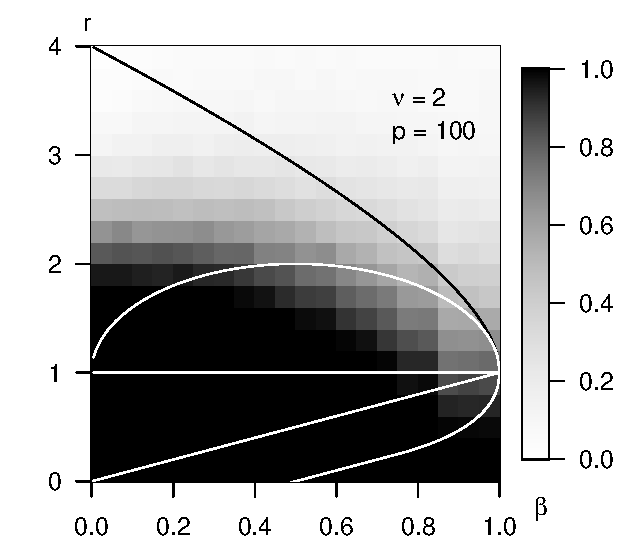
\includegraphics[width=0.32\textwidth]{./sim_approx-exact_boundary/simulated_approx-exact_boundary_chi-squared_nu2_p100.eps}
      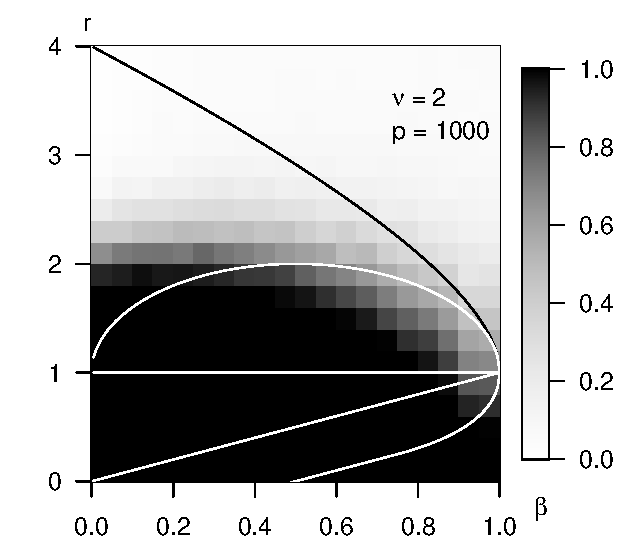
\includegraphics[width=0.32\textwidth]{./sim_approx-exact_boundary/simulated_approx-exact_boundary_chi-squared_nu2_p1000.eps}
      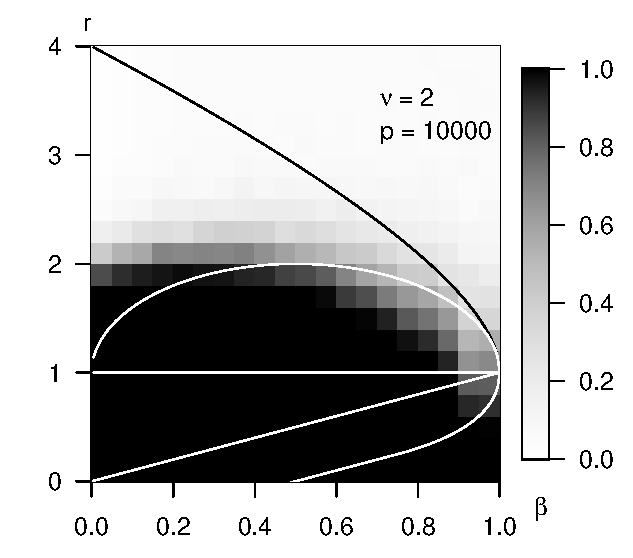
\includegraphics[width=0.32\textwidth]{./sim_approx-exact_boundary/simulated_approx-exact_boundary_chi-squared_nu2_p10000.eps}
      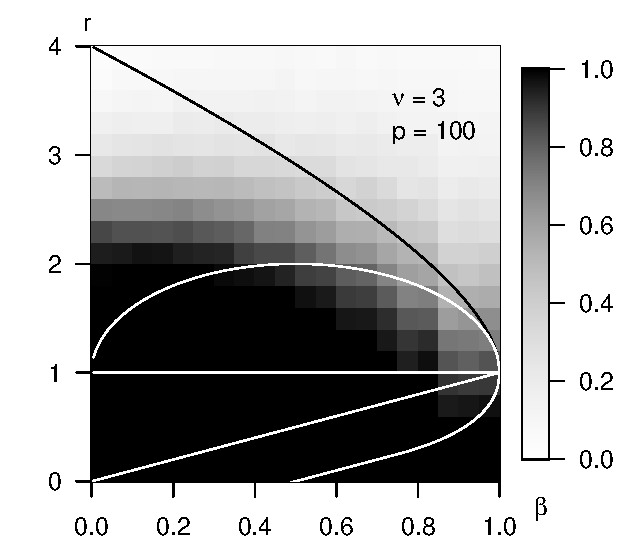
\includegraphics[width=0.32\textwidth]{./sim_approx-exact_boundary/simulated_approx-exact_boundary_chi-squared_nu3_p100.eps}
      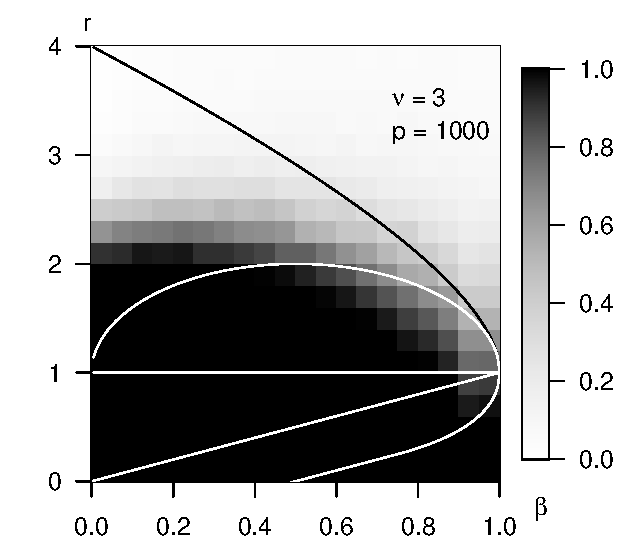
\includegraphics[width=0.32\textwidth]{./sim_approx-exact_boundary/simulated_approx-exact_boundary_chi-squared_nu3_p1000.eps}
      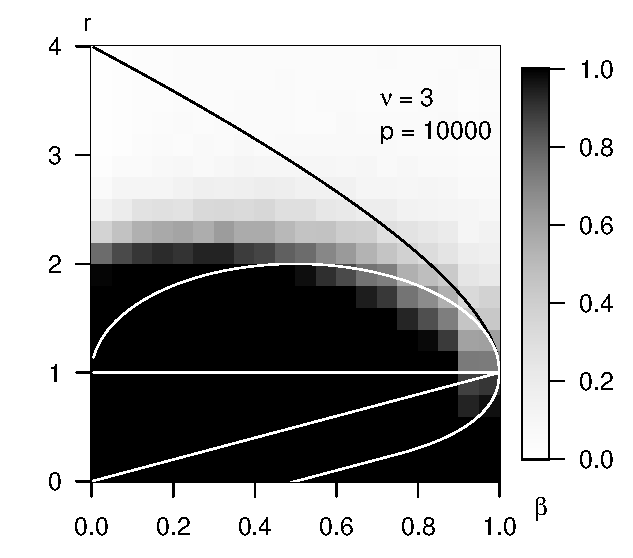
\includegraphics[width=0.32\textwidth]{./sim_approx-exact_boundary/simulated_approx-exact_boundary_chi-squared_nu3_p10000.eps}
      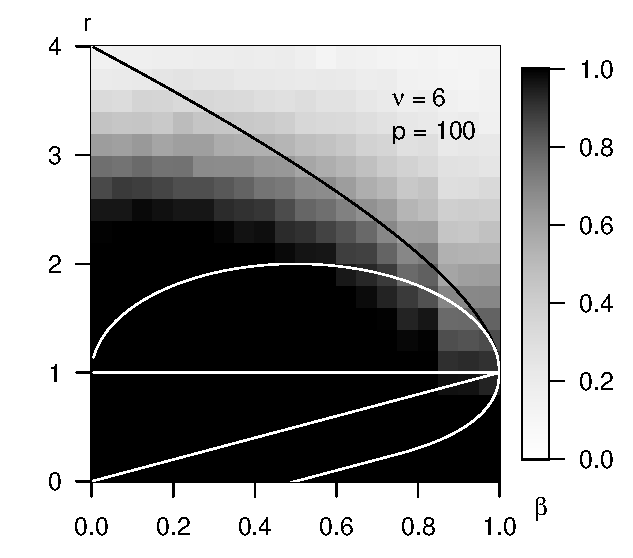
\includegraphics[width=0.32\textwidth]{./sim_approx-exact_boundary/simulated_approx-exact_boundary_chi-squared_nu6_p100.eps}
      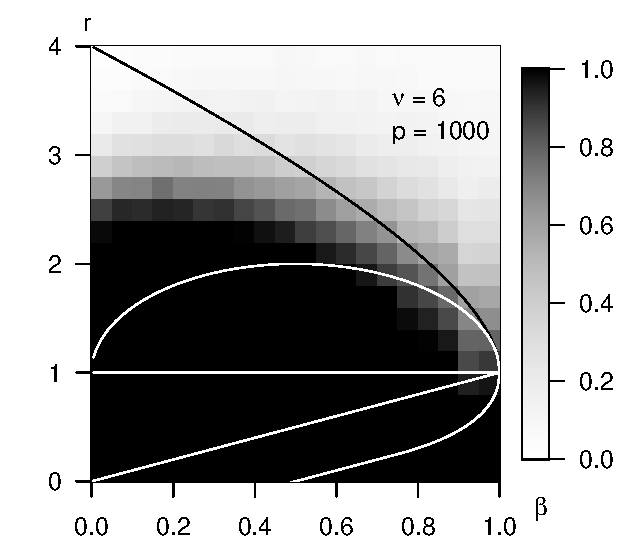
\includegraphics[width=0.32\textwidth]{./sim_approx-exact_boundary/simulated_approx-exact_boundary_chi-squared_nu6_p1000.eps}
      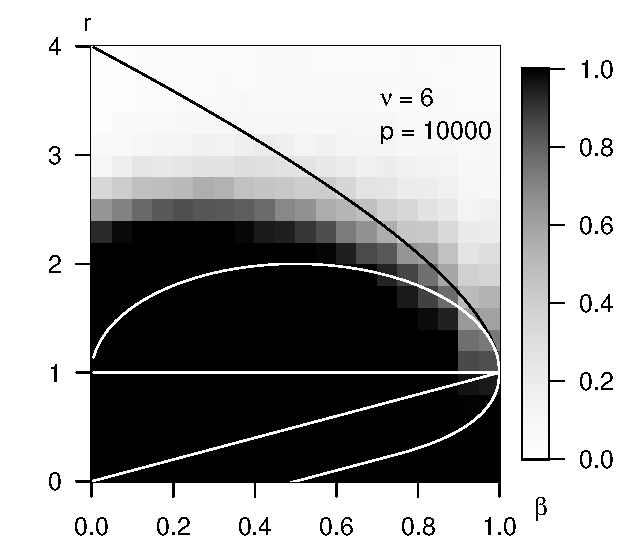
\includegraphics[width=0.32\textwidth]{./sim_approx-exact_boundary/simulated_approx-exact_boundary_chi-squared_nu6_p10000.eps}
      \caption{The estimated risk of approximate-exact support recovery $\mathrm{risk}^{\mathrm{EA}}$ (see \eqref{eq:risk-approx-exact}) of the Benjamini-Hochberg procedure in the chi-squared model \eqref{eq:model-chisq}. 
      We simulate $\nu=1, 2, 3, 6$ (first to last row), at dimensions $p=10^2, 10^3, 10^4$ (left to right column), for a grid of sparsity levels $\beta$ and signal sizes $r$.
      The experiments were repeated 1000 times for each sparsity-signal size combination; darker color indicates higher larger $\mathrm{risk}^{\mathrm{EA}}$. 
      Numerical results are generally in agreement with the boundaries described in Theorem \ref{thm:chi-squared-approx-boundary}; for small $\beta$'s and large $\nu$'s, the phase transitions take place somewhat above the predicted boundaries.
      Other boundaries in the support recovery and the detection problems are plotted for comparison.} 
      \label{fig:phase-simulated-chi-squared-approx-exact-boundary}
\end{figure}
